\documentclass[tikz,border=12pt]{standalone}
\usepackage{amsmath,amssymb}
\usetikzlibrary{arrows.meta,decorations.pathmorphing,calc}
\definecolor{ink}{HTML}{263145}
\definecolor{accent}{HTML}{4168B3}
\definecolor{warm}{HTML}{B77942}
\tikzset{every picture/.style={font=\small,text=ink},axis/.style={-{Stealth},thin,ink!65},curve/.style={accent,very thick},particle/.style={ink,thick,-{Stealth}}}
\begin{document}

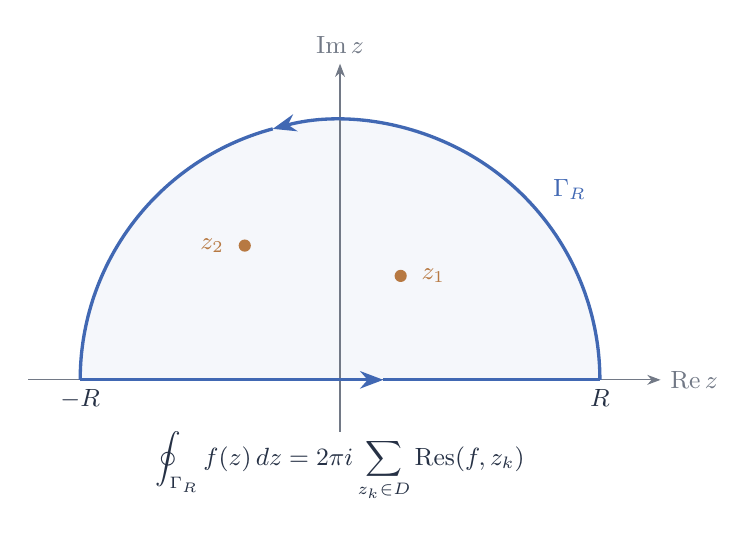
\begin{tikzpicture}[scale=1.1]
\fill[accent!5] (0,0)--(3,0) arc (0:180:3)--cycle;
\draw[axis] (-3.6,0)--(3.7,0) node[right] {$\operatorname{Re}z$};
\draw[axis] (0,-.6)--(0,3.65) node[above] {$\operatorname{Im}z$};
\draw[curve,-{Stealth}] (-3,0)--(.5,0);
\draw[curve] (.5,0)--(3,0);
\draw[curve,-{Stealth}] (3,0) arc (0:105:3);
\draw[curve] ({3*cos(105)},{3*sin(105)}) arc (105:180:3);
\fill[warm] (.7,1.2) circle (2pt) node[right=4pt] {$z_1$};
\fill[warm] (-1.1,1.55) circle (2pt) node[left=4pt] {$z_2$};
\node[below] at (-3,0) {$-R$};\node[below] at (3,0) {$R$};
\node[accent] at (2.65,2.2) {$\Gamma_R$};
\node at (0,-1) {$\displaystyle\oint_{\Gamma_R}f(z)\,dz=2\pi i\sum_{z_k\in D}\operatorname{Res}(f,z_k)$};
\end{tikzpicture}
\end{document}
